\chapter{Diagramas de Ellingham y metalurgia}\label{ch:b2:ellingham}

Un alto horno convierte una roca roja en hierro líquido con coque y aire caliente, a
razón de miles de toneladas al día. Ningún horno de ese tipo producirá nunca
aluminio, magnesio ni titanio, aunque el carbono sea igual de barato para ellos.
La mayoría de los metales se encuentran en el suelo como óxidos, y obtener un metal significa
quitarle su oxígeno: qué reductores pueden hacerlo, y a qué
temperatura, es una cuestión de \omterm{def:b2:reaction-free-energy:gibbs-energy}{energías de Gibbs} estándar. En 1944 Harold
Ellingham las representó todas en un mismo gráfico, en función de la temperatura, para un mol de
dioxígeno cada una. El gráfico responde de un vistazo qué metal reduce qué óxido,
por qué el carbono gana a alta temperatura y por qué algunos metales deben obtenerse por
electrólisis.

\begin{recall}
\Cref{ch:b2:reaction-free-energy}: $\Delta_r G^\circ = \Delta_r H^\circ -
T\Delta_r S^\circ$ y la \omterm{def:b2:reaction-free-energy:ellingham-approximation}{aproximación de Ellingham} (rectas en $T$,
salvo en los cambios de estado). \Cref{ch:b2:equilibrium-shifts}: $K^\circ$ a partir de
$\Delta_r G^\circ$, la \omterm{def:b2:equilibrium-shifts:variance}{varianza}, el fin de un equilibrio cuando desaparece una fase.
El volumen del primer año: números de oxidación, pares redox, óxidos básicos y
ácidos. El volumen escolar: las menas.
\end{recall}

\begin{omfigure}
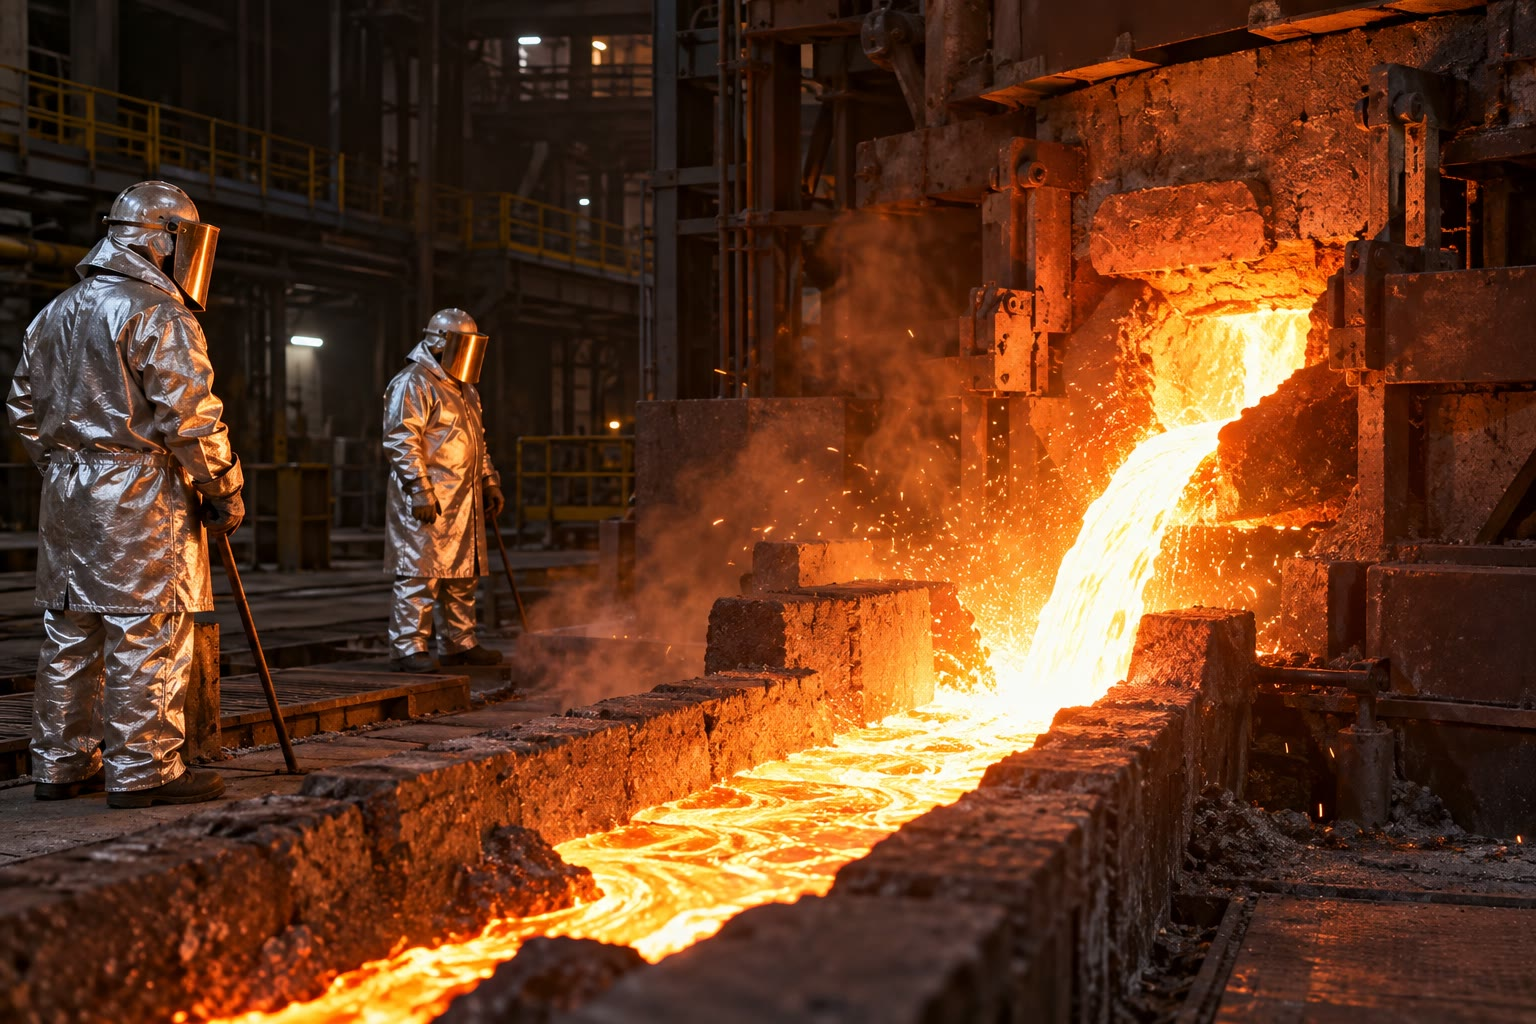
\includegraphics[width=0.62\linewidth]{images/book3/ai/b2-06-blast-furnace.jpg}

{\small Sangrado de un alto horno: el hierro líquido corre por un canal refractario,
vigilado por operarios con trajes que reflejan el calor. La temperatura y el gas
del interior del horno son los que permiten al monóxido de carbono quitarle el oxígeno
al óxido de hierro.}
\end{omfigure}

\section{El diagrama de Ellingham}

Para comparar la afinidad de distintos metales por el oxígeno, las reacciones se
escriben de modo que todas consuman la misma cantidad del reactivo común.

\begin{definition}[Diagrama de Ellingham]\label{def:b2:ellingham:diagram}
El \emph{diagrama de Ellingham}\index{diagrama de Ellingham} de una familia de óxidos
es la representación, en función de la temperatura, de las \omterm{def:b2:reaction-free-energy:gibbs-energy}{energías de Gibbs} estándar de sus
reacciones de formación escritas para un mol de dioxígeno,
\[
  \tfrac{2x}{y}\,\mathrm M + \ce{O2} \longrightarrow \tfrac{2}{y}\,\mathrm{M}_x\mathrm O_y ,
  \qquad \Delta_r G^\circ(T) \ \text{por mol de } \ce{O2} .
\]
\end{definition}

Por ejemplo, \ce{2Zn + O2 -> 2ZnO}, \ce{4/3Al + O2 -> 2/3Al2O3}, \ce{2C + O2 ->
2CO}. La ordenada está en \unit{kJ} por mol de \ce{O2}, siempre negativa para los
metales del gráfico.

\begin{proposition}[Rectas]\label{prop:b2:ellingham:line}
En la \omterm{def:b2:reaction-free-energy:ellingham-approximation}{aproximación de Ellingham}, cada línea es una recta de pendiente $-\Delta_r
S^\circ$. Para un metal y su óxido, ambos condensados, $\Delta_r S^\circ$ es
cercana a menos la entropía del mol de dioxígeno consumido, unos
$-\qty{200}{J/(K.mol)}$: las rectas suben con la temperatura, todas con casi la
misma pendiente.
\end{proposition}

\begin{proof}
$\Delta_r G^\circ = \Delta_r H^\circ - T\Delta_r S^\circ$ con $\Delta_r
H^\circ$ y $\Delta_r S^\circ$ constantes. Las entropías molares de los sólidos son de decenas de
\unit{J/(K.mol)} y se compensan en gran parte entre el metal y el óxido, mientras que se consume un mol de
gas, de entropía $S^\circ(\ce{O2}) = \qty{205}{J/(K.mol)}$. Para el cinc,
$2(43.65) - 2(41.63) - 205.15 = \qty{-201.1}{J/(K.mol)}$.
% ledger: s0:ZnO_cr, s0:Zn_cr, s0:O2_g
\end{proof}

\begin{proposition}[Cambios de pendiente]\label{prop:b2:ellingham:break}
A la temperatura a la que el metal funde o hierve, la recta cambia de pendiente:
su pendiente aumenta en $\nu\,\Delta_{\text{trs}}S$, donde $\nu$ es la cantidad de
metal en la reacción y $\Delta_{\text{trs}}S = \Delta_{\text{trs}}H/T_{\text{trs}}$.
Un cambio de estado del óxido disminuye, en cambio, la pendiente.
\end{proposition}

\begin{proof}
Por encima de la transición el metal reacciona desde su nueva fase, cuya entropía es
mayor en $\Delta_{\text{trs}}S$: $\Delta_r S^\circ$ disminuye en $\nu\,\Delta_{\text{trs}}S$
y la pendiente $-\Delta_r S^\circ$ aumenta otro tanto. La propia $\Delta_r G^\circ$
es continua, porque en $T_{\text{trs}}$ ambas fases tienen el mismo
\omterm{def:b2:chemical-potential:chemical-potential}{potencial químico}. Para el óxido, el signo es el opuesto.
\end{proof}

La fusión cambia poco la pendiente; la ebullición, que convierte un reactivo condensado
en un gas, la cambia mucho. El cinc hierve a \qty{1180}{K}: por encima de esa
temperatura la formación del óxido de cinc consume tres moles de gas por cada dos de
óxido, y su recta sube con fuerza. Lo mismo le ocurre al magnesio por encima de su
punto de ebullición.

\begin{omfigure}
\begin{tikzpicture}[lab/.style={anchor=west, font=\scriptsize, inner sep=1pt}]
\begin{axis}[omellingham,
  width=0.84\linewidth, height=11cm, xmin=300, xmax=2100, ymin=-1250, ymax=0,
  clip mode=individual,
  xlabel={$T$ (K)}, ylabel={$\Delta_r G^\circ$ (\unit{kJ} por mol de \ce{O2})},
  xtick={300,500,700,900,1100,1300,1500,1700,1900,2100},
  x tick label style={rotate=45, anchor=north east, font=\scriptsize}]
\addplot[black!60, thick] table[x=T, y=G] {figdata/out/bachelor-2-ellingham-a-HgO.dat};
\addplot[omProp, thick] table[x=T, y=G] {figdata/out/bachelor-2-ellingham-a-Cu2O.dat};
\addplot[omDef, thick] table[x=T, y=G] {figdata/out/bachelor-2-ellingham-a-FeO.dat};
\addplot[omExo, very thick] table[x=T, y=G] {figdata/out/bachelor-2-ellingham-a-ZnO.dat};
\addplot[black!60, thick] table[x=T, y=G] {figdata/out/bachelor-2-ellingham-a-Cr2O3.dat};
\addplot[omProp, thick] table[x=T, y=G] {figdata/out/bachelor-2-ellingham-a-TiO2.dat};
\addplot[omDef, thick] table[x=T, y=G] {figdata/out/bachelor-2-ellingham-a-Al2O3.dat};
\addplot[black!60, thick] table[x=T, y=G] {figdata/out/bachelor-2-ellingham-a-MgO.dat};
\addplot[omProp, thick] table[x=T, y=G] {figdata/out/bachelor-2-ellingham-a-CaO.dat};
\addplot[omThm, very thick] table[x=T, y=G] {figdata/out/bachelor-2-ellingham-a-C-CO.dat};
\addplot[omThm, thick, dashed] table[x=T, y=G] {figdata/out/bachelor-2-ellingham-a-C-CO2.dat};
\addplot[omThm, thick, dotted] table[x=T, y=G] {figdata/out/bachelor-2-ellingham-a-CO-CO2.dat};
\addplot[omDef, thick, dashed] table[x=T, y=G] {figdata/out/bachelor-2-ellingham-a-H2-H2O.dat};
% labels: inside for the two short lines, at the right end for the others
\node[font=\scriptsize, black!70, anchor=south] at (axis cs:400,-60) {\ce{HgO}};
\node[font=\scriptsize, omProp, anchor=south] at (axis cs:1100,-150) {\ce{Cu2O}};
\draw[omExo, thin] (axis cs:2100,-69) -- (axis cs:2150,-60) node[lab, text=omExo] {\ce{ZnO}};
\draw[omThm, thin] (axis cs:2100,-204) -- (axis cs:2150,-185) node[lab, text=omThm] {\ce{CO}/\ce{CO2}};
\draw[omDef, thin] (axis cs:2100,-259) -- (axis cs:2150,-235) node[lab, text=omDef] {\ce{H2}/\ce{H2O}};
\draw[omDef, thin] (axis cs:2100,-286) -- (axis cs:2150,-285) node[lab, text=omDef] {\ce{FeO}};
\draw[black!70, thin] (axis cs:2100,-393) -- (axis cs:2150,-365) node[lab, text=black!70] {\ce{Cr2O3}};
\draw[omThm, thin] (axis cs:2100,-396) -- (axis cs:2150,-415) node[lab, text=omThm] {\ce{C}/\ce{CO2}};
\draw[omProp, thin] (axis cs:2100,-567) -- (axis cs:2150,-540) node[lab, text=omProp] {\ce{TiO2}};
\draw[omThm, thin] (axis cs:2100,-589) -- (axis cs:2150,-590) node[lab, text=omThm] {\ce{C}/\ce{CO}};
\draw[black!70, thin] (axis cs:2100,-600) -- (axis cs:2150,-640) node[lab, text=black!70] {\ce{MgO}};
\draw[omDef, thin] (axis cs:2100,-668) -- (axis cs:2150,-690) node[lab, text=omDef] {\ce{Al2O3}};
\draw[omProp, thin] (axis cs:2100,-765) -- (axis cs:2150,-765) node[lab, text=omProp] {\ce{CaO}};
\end{axis}
\end{tikzpicture}

{\small El \omterm{def:b2:ellingham:diagram}{diagrama de Ellingham}: \omterm{def:b2:reaction-free-energy:gibbs-energy}{energía de Gibbs} estándar de formación de los óxidos
por mol de \ce{O2}, en función de la temperatura, a partir de \omterm{def:b2:reaction-free-energy:gibbs-energy}{energías de Gibbs} tabuladas. Cuanto
más baja es una recta, más estable es el óxido y más reductor es el metal.
Cada recta de metal lleva el nombre de su óxido; \ce{C}/\ce{CO} es \ce{2C + O2 -> 2CO},
\ce{C}/\ce{CO2} es \ce{C + O2 -> CO2}, \ce{CO}/\ce{CO2} es \ce{2CO + O2 -> 2CO2}
y \ce{H2}/\ce{H2O} es \ce{2H2 + O2 -> 2H2O}, con el agua gaseosa.}
% ledger: janafG:Cu2O.300, janafG:FeO.300, janafG:Cr2O3.300, janafG:TiO2.500, janafG:Al2O3.300, janafG:MgO.300, janafG:CaO.300, janafG:CO.300, janafG:CO2.300, janafG:H2O.300, dfh:ZnO_cr, dfh:HgO_cr, s0:HgO_cr, s0:Hg_l, s0:Hg_g, dfh:Hg_g (all temperatures in figdata/bachelor-2/ellingham.py)
\end{omfigure}

\section{Lectura del diagrama}

\begin{definition}[Presión de oxígeno de equilibrio]\label{def:b2:ellingham:oxygen-pressure}
La \emph{presión de oxígeno de equilibrio}\index{presion de oxigeno de equilibrio@presión de oxígeno de equilibrio} de un
par metal–óxido a la temperatura $T$ es la presión de dioxígeno a la que el metal
y el óxido coexisten en equilibrio: $RT\ln(p_{\ce{O2}}/p^\circ) = \Delta_r
G^\circ(T)$ para la reacción escrita por mol de \ce{O2}.
\end{definition}

\begin{theorem}[Dominios del metal y del óxido]\label{thm:b2:ellingham:domains}
En una atmósfera de presión de oxígeno $p_{\ce{O2}}$ a la temperatura $T$, el
metal se oxida si $RT\ln(p_{\ce{O2}}/p^\circ) > \Delta_r G^\circ(T)$, y el
óxido se reduce a metal si $RT\ln(p_{\ce{O2}}/p^\circ) < \Delta_r
G^\circ(T)$. En el diagrama, el óxido es estable por encima de su recta, y el metal,
por debajo.
\end{theorem}

\begin{proof}
Con el metal y el óxido condensados, de actividad 1, $Q = p^\circ/p_{\ce{O2}}$ y
$\Delta_r G = \Delta_r G^\circ + RT\ln Q = \Delta_r G^\circ - RT\ln(p_{\ce{O2}}/
p^\circ)$. La oxidación avanza en sentido directo cuando $\Delta_r G < 0$.
\end{proof}

En el aire ($p_{\ce{O2}} = \qty{0.21}{bar}$; $RT\ln 0.21$ vale \qty{-4}{kJ/mol}
a temperatura ambiente y \qty{-13}{kJ/mol} a \qty{1000}{K}, casi cero a esta
escala) se oxida todo metal del diagrama cuya recta
esté por debajo del eje: a temperatura ambiente, todos, incluso el cobre.
Solo los óxidos cercanos a la parte superior (plata, mercurio) se descomponen con un
calentamiento moderado.

\begin{example}[El óxido de mercurio]\label{ex:b2:ellingham:hgo}
Para \ce{2Hg + O2 -> 2HgO}, los valores clave del CODATA dan $\Delta_r H^\circ =
\qty{-181.6}{kJ/mol}$ con mercurio líquido; por encima del punto de ebullición del mercurio
el metal es un gas y $\Delta_r H^\circ = \qty{-304.3}{kJ/mol}$, $\Delta_r
S^\circ = \qty{-414.6}{J/(K.mol)}$. La recta corta el cero en
$T = 304.3/0.4146 \approx \qty{734}{K}$: calentado por encima de esa temperatura en aire,
o bajo \qty{1}{bar} de oxígeno, el óxido rojo de mercurio desprende su oxígeno
---así se aisló el oxígeno por primera vez, en 1774---.
% ledger: dfh:HgO_cr, s0:HgO_cr, s0:Hg_l, s0:Hg_g, dfh:Hg_g, s0:O2_g (computed in figdata/bachelor-2/ellingham.py)
\end{example}

\begin{proposition}[Qué metal reduce qué óxido]\label{prop:b2:ellingham:reduction}
A una temperatura dada, un metal M reduce el óxido de un metal N, en
condiciones estándar, cuando la recta de M está por debajo de la de N. La \omterm{def:b2:reaction-free-energy:reaction-gibbs}{energía de Gibbs
estándar de reacción} de la reducción, por mol de \ce{O2} transferido, es la
diferencia de las dos ordenadas.
\end{proposition}

\begin{proof}
La reducción es la formación del óxido de M menos la del óxido de N, ambas por
mol de \ce{O2}: $\Delta_r G^\circ = \Delta_r G^\circ_{\mathrm M} - \Delta_r
G^\circ_{\mathrm N}$, negativa cuando la recta de M es más baja.
\end{proof}

\begin{method}[Leer un diagrama de Ellingham]\label{met:b2:ellingham:read-ellingham}
\begin{enumerate}
  \item Búsquense las dos rectas a la temperatura que interesa. La más baja corresponde
        al óxido más estable; su metal reduce el otro óxido.
  \item La distancia vertical es $\Delta_r G^\circ$ por mol de \ce{O2}: una distancia de
        \qty{100}{kJ} o más significa una reducción prácticamente completa.
  \item Donde dos rectas se cortan, la reducción cambia de sentido: léase la
        temperatura del cruce.
  \item Atención a los cambios de pendiente: un metal que hierve dentro del intervalo sale como
        vapor, que puede separarse por destilación o bien reoxidarse al enfriarse.
\end{enumerate}
\end{method}

\begin{definition}[Reducción aluminotérmica]\label{def:b2:ellingham:aluminothermy}
Una \emph{reducción aluminotérmica}\index{reduccion aluminotermica@reducción aluminotérmica} es la
reducción de un óxido metálico por aluminio en polvo, posible para todo óxido cuya
recta esté por encima de la de la alúmina, y tan \omterm{def:b2:reaction-enthalpy:exothermic}{exotérmica} que la mezcla funde:
\ce{Fe2O3 + 2Al -> Al2O3 + 2Fe} (termita) suelda raíles; \ce{Cr2O3 + 2Al ->
Al2O3 + 2Cr} produce cromo libre de carbono.
\end{definition}

\begin{omfigure}
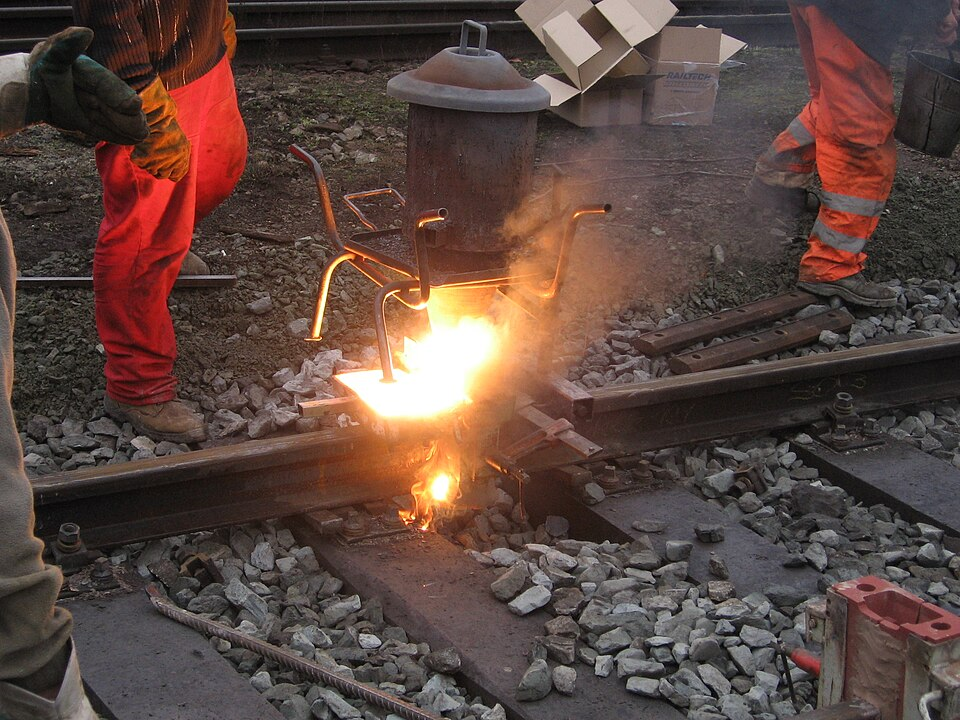
\includegraphics[width=0.5\linewidth]{images/book3/thermite.jpg}

{\small Soldadura aluminotérmica de un raíl: la reacción del óxido de hierro con el aluminio
en el crisol situado sobre la junta da hierro líquido, que baja al
molde entre los dos extremos del raíl. (Fotografía: PetrS., CC BY-SA 3.0, Wikimedia
Commons.)}
\end{omfigure}

\section{El carbono y el monóxido de carbono}

Tres rectas involucran al carbono:
\begin{itemize}
  \item \ce{C + O2 -> CO2}: un mol de gas da uno, $\Delta_r S^\circ
        \approx 0$, una recta casi horizontal cerca de \qty{-395}{kJ};
  \item \ce{2C + O2 -> 2CO}: un mol de gas da dos, $\Delta_r S^\circ
        \approx \qty{+180}{J/(K.mol)}$, una recta que \emph{desciende} con la temperatura;
  \item \ce{2CO + O2 -> 2CO2}: tres moles de gas dan dos, una recta ascendente.
\end{itemize}

\begin{proposition}[El carbono lo reduce casi todo en caliente]\label{prop:b2:ellingham:carbon}
La recta de \ce{2C + O2 -> 2CO} desciende con la temperatura y corta las
rectas de la mayoría de los óxidos metálicos: por encima de la temperatura de cruce, el carbono reduce el
óxido y da monóxido de carbono. El cruce con el óxido de hierro(II) está cerca de
\qty{1040}{K}, con el óxido de cinc cerca de \qty{1220}{K}; para el óxido de titanio y la magnesia
está cerca de \qty{2000}{K} o por encima, y para la alúmina, más arriba aún, donde los metales
se combinan con el carbono en carburos o se reoxidan al enfriarse el gas.
\end{proposition}

\begin{proof}
La pendiente $-\Delta_r S^\circ$ de la recta del carbono es negativa ($\Delta\nu_{\text{gas}}
= +1$), y la de las rectas de los óxidos, positiva: se cortan una sola vez. Las temperaturas
se leen en las rectas calculadas.
% ledger: janafG:CO.900, janafG:CO.1100, janafG:FeO.900, janafG:FeO.1100 (crossings computed in figdata/bachelor-2/ellingham.py)
\end{proof}

\begin{definition}[Equilibrio de Boudouard]\label{def:b2:ellingham:boudouard}
El \emph{equilibrio de Boudouard}\index{equilibrio de Boudouard} es \ce{C(s) + CO2(g) <=> 2CO(g)},
\omterm{def:b2:reaction-enthalpy:exothermic}{endotérmico}, entre el carbono y los dos óxidos de carbono.
\end{definition}

\begin{proposition}[Composición del gas sobre el carbono]\label{prop:b2:ellingham:boudouard}
El sistema carbono + \ce{CO} + \ce{CO2} tiene \omterm{def:b2:equilibrium-shifts:variance}{varianza} 2: a $T$ y presión total
$p$ dadas, la fracción molar $x$ de monóxido de carbono queda fijada por $x^2/(1 - x)
= K^\circ(T)\,p^\circ/p$. A \qty{1}{bar} el gas es casi \ce{CO2} puro
por debajo de \qty{700}{K} y casi \ce{CO} puro por encima de \qty{1200}{K}; el cruce de
las tres rectas del carbono, cerca de \qty{975}{K}, es donde $K^\circ = 1$.
\end{proposition}

\begin{proof}
Tres especies, una reacción, dos fases: $v = 3 - 1 + 2 - 2 = 2$. Con $p_{\ce{CO}}
= xp$ y $p_{\ce{CO2}} = (1 - x)p$, $Q = x^2p/[(1 - x)p^\circ]$. Cuando $K^\circ = 1$,
las \omterm{def:b2:reaction-free-energy:gibbs-energy}{energías de Gibbs} estándar de \ce{2C + O2 -> 2CO} y de \ce{C + O2 -> CO2} son
iguales: las dos rectas, y por tanto la tercera, se cortan.
\end{proof}

\begin{omfigure}
\begin{tikzpicture}
\begin{axis}[
  width=0.62\linewidth, height=5.4cm, xmin=500, xmax=1500, ymin=0, ymax=1.05,
  axis x line=bottom, axis y line=left, xlabel={$T$ (K)},
  xtick={500,700,900,1100,1300,1500}, ytick={0,0.5,1},
  ylabel={fracción molar de \ce{CO}}, tick label style={font=\small},
  label style={font=\small}, clip=false]
\addplot[omThm, very thick] table[x=T, y=xCO] {figdata/out/bachelor-2-ellingham-b.dat};
\node[font=\scriptsize, anchor=west] at (axis cs:1150,0.55) {\ce{CO} estable};
\node[font=\scriptsize, anchor=west] at (axis cs:510,0.6) {\ce{CO2} (y carbono) estable};
\end{axis}
\end{tikzpicture}

{\small El \omterm{def:b2:ellingham:boudouard}{equilibrio de Boudouard} a \qty{1}{bar}: fracción molar de monóxido
de carbono en un gas en equilibrio con carbono.}
% ledger: janafG:CO.700, janafG:CO2.700, janafG:CO.1100, janafG:CO2.1100 (computed in figdata/bachelor-2/ellingham.py)
\end{omfigure}

\section{El alto horno}

El mineral de hierro (hematites \ce{Fe2O3}, magnetita \ce{Fe3O4}), el coque y la caliza se
cargan por la parte superior de una cuba alta; por la parte baja se insufla aire
caliente. Al bajar, los sólidos encuentran un gas caliente ascendente; el gas sale
por arriba, enfriado.
\begin{itemize}
  \item En las toberas, el coque arde en el aire caliente: \ce{C + O2 -> CO2}, y
        más arriba, con exceso de carbono, \ce{CO2 + C -> 2CO} (Boudouard): el gas
        que sube es sobre todo monóxido de carbono y nitrógeno.
  \item En la parte superior, el monóxido de carbono reduce los óxidos de hierro etapa por
        etapa, \ce{3Fe2O3 + CO -> 2Fe3O4 + CO2}, \ce{Fe3O4 + CO -> 3FeO + CO2},
        \ce{FeO + CO -> Fe + CO2}. Las dos primeras etapas son fáciles; para la última,
        la recta \ce{CO}/\ce{CO2} pasa un poco \textit{por encima} de la recta de
        \ce{FeO}: su \omterm{def:b2:reaction-free-energy:reaction-gibbs}{energía de Gibbs estándar de reacción} es ligeramente positiva
        ($K^\circ \approx 0.3$ a \qty{900}{K}), y la reducción necesita un gas
        con al menos tres veces más \ce{CO} que \ce{CO2}, que es lo que
        proporciona el \omterm{def:b2:ellingham:boudouard}{equilibrio de Boudouard} en la zona caliente inferior.
  \item Más abajo y más caliente, el propio carbono reduce lo que queda, \ce{FeO + C ->
        Fe + CO}; el hierro disuelve carbono, funde y se acumula en el fondo
        con una escoria fundida formada por la cal y la sílice del mineral.
\end{itemize}

\begin{omfigure}
\begin{tikzpicture}[font=\small, >={Stealth}]
  \fill[gray!12] (-1.4,0) -- (-2.0,3.0) -- (-1.3,7.0) -- (1.3,7.0) -- (2.0,3.0) -- (1.4,0) -- cycle;
  \draw[thick] (-1.4,0) -- (-2.0,3.0) -- (-1.3,7.0) (1.4,0) -- (2.0,3.0) -- (1.3,7.0);
  \draw[thick] (-1.4,0) -- (1.4,0);
  \fill[orange!70!red] (-1.4,0) rectangle (1.4,0.35);
  \fill[yellow!50!orange] (-1.45,0.35) rectangle (1.45,0.6);
  \node[font=\scriptsize] at (0,0.17) {hierro líquido};
  \node[font=\scriptsize] at (0,0.48) {escoria};
  % tuyeres
  \draw[->, thick, omDef] (-3.2,1.2) -- (-1.75,1.2) node[pos=0, left] {aire caliente};
  \draw[->, thick, omDef] (3.2,1.2) -- (1.75,1.2);
  % charge and gas
  \draw[->, thick] (-0.6,7.9) -- (-0.6,7.1) node[pos=0, above left, xshift=6pt] {mineral, coque, caliza};
  \draw[->, thick, omThm] (0.7,7.1) -- (0.7,7.9) node[pos=1, above right, xshift=-6pt] {gas de tragante (\ce{CO}, \ce{CO2}, \ce{N2})};
  \draw[->, omThm, thick] (0.6,1.6) -- (0.6,6.4);
  \draw[->, thick] (-0.6,6.4) -- (-0.6,1.6);
  \node[omThm, font=\scriptsize, rotate=90] at (0.9,4.0) {el gas sube};
  \node[font=\scriptsize, rotate=90] at (-0.9,4.0) {los sólidos bajan};
  % zones
  \node[anchor=west, align=left, font=\scriptsize] at (2.3,6.0) {\ce{3Fe2O3 + CO -> 2Fe3O4 + CO2}\\ \ce{Fe3O4 + CO -> 3FeO + CO2}};
  \node[anchor=west, align=left, font=\scriptsize] at (2.3,4.2) {\ce{FeO + CO -> Fe + CO2}};
  \node[anchor=west, align=left, font=\scriptsize] at (2.3,2.7) {\ce{CO2 + C -> 2CO}\\ \ce{FeO + C -> Fe + CO}};
  \node[anchor=west, align=left, font=\scriptsize] at (2.3,1.6) {\ce{C + O2 -> CO2}};
  \draw[densely dotted] (1.95,6.0) -- (2.3,6.0) (1.9,4.2) -- (2.3,4.2) (2.0,2.8) -- (2.3,2.8);
  \node[anchor=east, align=right, font=\scriptsize, black!60] at (-2.2,6.0) {más frío};
  \node[anchor=east, align=right, font=\scriptsize, black!60] at (-2.2,2.3) {más caliente};
  \draw[->, black!50] (-2.6,5.6) -- (-2.6,2.7);
\end{tikzpicture}

{\small El alto horno como reactor a contracorriente. Los sólidos bajan y el gas
reductor caliente sube; los óxidos de hierro se reducen con monóxido de carbono en la
parte superior, más fría, y con carbono en la parte inferior, más caliente. El hierro y la escoria
se sangran por el fondo.}
\end{omfigure}

\begin{omfigure}
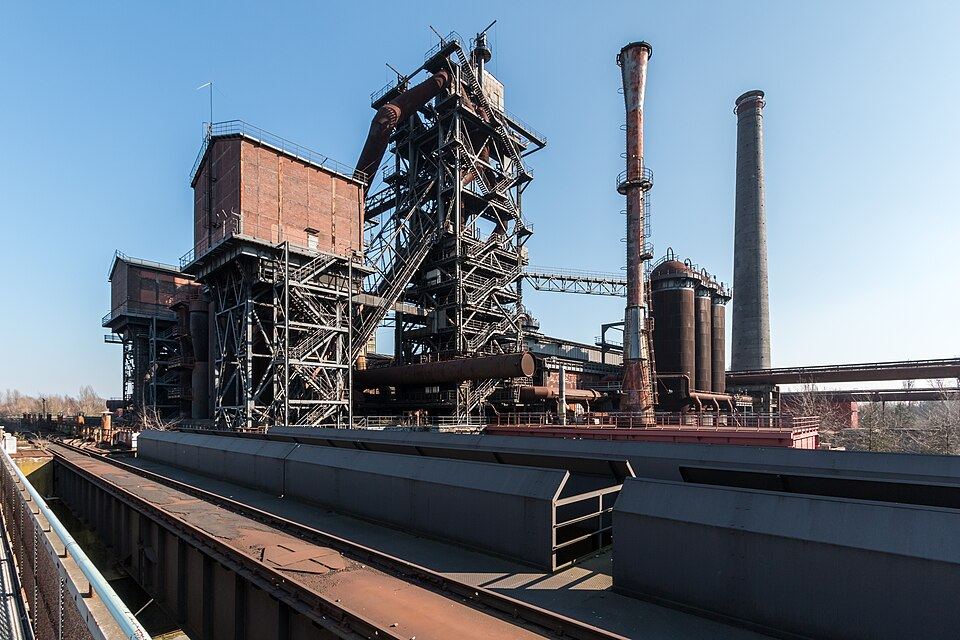
\includegraphics[width=0.6\linewidth]{images/book3/blast-furnace.jpg}

{\small Un alto horno conservado como monumento (Duisburg-Nord, cerrado en
1985): la cuba alta con su anillo de tuberías para el aire caliente y las tomas de gas
en la parte superior. (Fotografía: Dietmar Rabich, CC BY-SA 4.0, Wikimedia Commons.)}
\end{omfigure}

\section{Otras vías hacia un metal}

\begin{definition}[Pirometalurgia e hidrometalurgia]\label{def:b2:ellingham:metallurgy}
La \emph{pirometalurgia}\index{pirometalurgia} extrae un metal a alta
temperatura, por reducción de su óxido en un horno. La \emph{hidrometalurgia}\index{hidrometalurgia}
lo extrae de una disolución acuosa. Sus etapas habituales son la
\emph{tostación}\index{tostacion@tostación} (calentar en aire una mena sulfurada para convertirla en
un óxido, \ce{2ZnS + 3O2 -> 2ZnO + 2SO2}), la \emph{lixiviación}\index{lixiviacion@lixiviación}
(disolver el compuesto del metal, a menudo en ácido sulfúrico, \ce{ZnO + 2H+ ->
Zn^2+ + H2O}), la purificación de la disolución, por ejemplo por
\emph{cementación}\index{cementacion@cementación} (reducción de los iones de un metal más noble
por el polvo de uno menos noble, \ce{Cu^2+ + Zn -> Cu + Zn^2+}), y la
recuperación del metal, a menudo por electrólisis.
\end{definition}

El diagrama explica el reparto de tareas. El hierro, el cinc, el plomo y el estaño se obtienen con
carbono en un horno. El aluminio, cuya recta está muy por debajo de la del carbono a cualquier
temperatura practicable, se obtiene por electrólisis de su óxido fundido
(\cref{ch:b2:batteries-electrolysis}); el magnesio, por electrólisis o por
reducción con silicio a vacío, que elimina el vapor de magnesio;
el titanio, convirtiendo el óxido en cloruro, \ce{TiO2 + 2Cl2 + C -> TiCl4 +
CO2} (\cref{exo:b2:reaction-free-energy:12}), y reduciendo después el cloruro con
magnesio (el proceso Kroll). La mayor parte del cinc del mundo se obtiene por \omterm{def:b2:ellingham:metallurgy}{tostación},
\omterm{def:b2:ellingham:metallurgy}{lixiviación} y electrólisis: la vía hidrometalúrgica da un metal más puro y
evita manipular vapor de cinc.

\begin{omfigure}
\begin{tikzpicture}[font=\small, >={Stealth}, box/.style={draw, thick, rounded corners=2pt, align=center, minimum height=0.9cm, fill=white, text width=2.3cm}]
  \node[box] (r) at (0,0) {tostación\\ \ce{ZnS} $\to$ \ce{ZnO}};
  \node[box] (l) at (3.2,0) {lixiviación\\ en \ce{H2SO4}};
  \node[box] (c) at (6.4,0) {purificación\\ (cementación)};
  \node[box] (e) at (9.6,0) {electrólisis\\ \ce{Zn^2+} $\to$ \ce{Zn}};
  \draw[->, thick] (r) -- (l); \draw[->, thick] (l) -- (c); \draw[->, thick] (c) -- (e);
  \draw[->, thick, black!60] (r.north) -- ++(0,0.7) node[above] {\ce{SO2} $\to$ ácido sulfúrico};
  \draw[->, thick, omThm] (e.south) -- ++(0,-0.6) -| (l.south) node[pos=0.25, below] {ácido recirculado};
  \draw[->, thick] (e.east) -- ++(0.8,0) node[right] {cinc};
\end{tikzpicture}

{\small La vía hidrometalúrgica del cinc. El dióxido de azufre del horno de \omterm{def:b2:ellingham:metallurgy}{tostación}
se convierte en el ácido sulfúrico de la \omterm{def:b2:ellingham:metallurgy}{lixiviación}; el ácido regenerado en el
ánodo de la electrólisis vuelve a ella.}
\end{omfigure}

\section{Ejercicios}

\begin{exercise}[$\star$]\label{exo:b2:ellingham:1}
Escríbanse las reacciones representadas por las rectas del óxido de cobre(I), de la alúmina, del
monóxido de carbono y del dióxido de carbono, cada una para un mol de \ce{O2}.
\end{exercise}

\begin{exercise}[$\star$]\label{exo:b2:ellingham:2}
A partir de los valores clave del CODATA ($\Delta_f H^\circ(\ce{ZnO}) = \qty{-350.46}{kJ/mol}$;
$S^\circ$: \ce{ZnO} 43.65, \ce{Zn} 41.63, \ce{O2} \qty{205.15}{J/(K.mol)}),
escríbase $\Delta_r G^\circ(T)$ de \ce{2Zn + O2 -> 2ZnO} para el cinc sólido.
\end{exercise}

\begin{exercise}[$\star$]\label{exo:b2:ellingham:3}
Con el diagrama, enumérense los metales que pueden reducir el óxido de cromo(III) a
\qty{1500}{K} y los que no pueden.
\end{exercise}

\begin{exercise}[$\star$]\label{exo:b2:ellingham:4}
Explíquese el signo de la pendiente de cada una de las tres rectas del carbono.
\end{exercise}

\begin{exercise}[$\star\star$]\label{exo:b2:ellingham:5}
Calcúlese la \omterm{def:b2:ellingham:oxygen-pressure}{presión de oxígeno de equilibrio} del óxido de mercurio(II) a \qty{600}{K}
(mercurio líquido, $\Delta_r H^\circ = \qty{-181.6}{kJ}$, $\Delta_r S^\circ =
\qty{-216.5}{J/K}$ por mol de \ce{O2}). ¿Se oxida el mercurio en el aire a esa
temperatura?
\end{exercise}

\begin{exercise}[$\star\star$]\label{exo:b2:ellingham:6}
Calcúlese $\Delta_r G^\circ$ a \qty{298}{K} de la reacción de la termita, \ce{Fe2O3 +
2Al -> Al2O3 + 2Fe}, sabiendo que $\Delta_f G^\circ = \qty{-743.5}{kJ/mol}$ para
\ce{Fe2O3} y \qty{-1582.3}{kJ/mol} para \ce{Al2O3}, y dígase por qué la reacción,
aunque muy \omterm{def:b2:reaction-free-energy:exergonic}{exergónica}, no empieza a temperatura ambiente.
% ledger: janafG:Fe2O3.298, janafG:Al2O3.298
\end{exercise}

\begin{exercise}[$\star\star$]\label{exo:b2:ellingham:7}
Hállese en el diagrama la temperatura por encima de la cual el carbono reduce el óxido de hierro(II)
a hierro con formación de monóxido de carbono, y escríbase la reacción.
\end{exercise}

\begin{exercise}[$\star\star$]\label{exo:b2:ellingham:8}
A \qty{1100}{K}, $\Delta_f G^\circ(\ce{CO}) = \qty{-209.1}{kJ/mol}$ y
$\Delta_f G^\circ(\ce{CO2}) = \qty{-396.0}{kJ/mol}$. Calcúlense la $K^\circ$ del
\omterm{def:b2:ellingham:boudouard}{equilibrio de Boudouard} y la fracción molar de monóxido de carbono sobre carbono a
\qty{1}{bar}. ¿Qué le ocurre al gas, en contacto con hollín o con hierro, cuando se
enfría a \qty{700}{K}?
% ledger: janafG:CO.1100, janafG:CO2.1100
\end{exercise}

\begin{exercise}[$\star\star$]\label{exo:b2:ellingham:9}
A veces se usa hidrógeno para reducir el óxido de wolframio. Con la recta del agua,
explíquese por qué el hidrógeno es mejor reductor que el monóxido de carbono a alta
temperatura pero peor a baja temperatura.
\end{exercise}

\begin{exercise}[$\star\star\star$]\label{exo:b2:ellingham:10}
El óxido de magnesio puede reducirse con silicio, \ce{2MgO + Si -> SiO2 + 2Mg}, aunque
la recta de la sílice está por encima de la de la magnesia a todas las temperaturas del
diagrama. A \qty{1500}{K}, el magnesio es un gas y las tablas dan, por mol de
\ce{O2}, \qty{-845.5}{kJ} para la magnesia y \qty{-643.7}{kJ} para la sílice.
Calcúlese $\Delta_r G^\circ$ de la reducción y luego la presión de vapor de
magnesio por debajo de la cual avanza en sentido directo. ¿Cómo aprovecha esto un horno de vacío?
% ledger: janafG:MgO.1500, janafG:SiO2.1500
\end{exercise}

\begin{exercise}[$\star\star\star$]\label{exo:b2:ellingham:11}
Calcúlese la \omterm{def:b2:equilibrium-shifts:variance}{varianza} del sistema \ce{FeO(s)}, \ce{Fe(s)}, \ce{CO(g)},
\ce{CO2(g)} en equilibrio. ¿Qué significa para el gas que sale de la parte superior
de un alto horno?
\end{exercise}

\begin{exercise}[$\star\star\star$]\label{exo:b2:ellingham:12}
El cobre se purifica de su disolución de \omterm{def:b2:ellingham:metallurgy}{lixiviación} por \omterm{def:b2:ellingham:metallurgy}{cementación} con chatarra de hierro.
Con los potenciales estándar del volumen del primer año ($E^\circ(\ce{Cu^2+}/\ce{Cu})
= \qty{0.34}{V}$, $E^\circ(\ce{Fe^2+}/\ce{Fe}) = \qty{-0.41}{V}$), calcúlense la
constante de equilibrio de \ce{Cu^2+ + Fe -> Cu + Fe^2+} y la concentración
residual de iones cobre cuando la disolución contiene \qty{1.0}{mol/L} de
\ce{Fe^2+}.
\end{exercise}

\section{Problema: el cinc por el fuego}

\begin{problem}[{Problema de fin de semana --- las rectas de Ellingham del óxido de cinc y del
monóxido de carbono, la temperatura a la que el carbono reduce el óxido de cinc, la
varianza del horno y la condensación del vapor de cinc}]
\label{pb:b2:ellingham:1}
Antes de la electrólisis, el cinc se obtenía calentando su óxido con carbono en retortas
de arcilla. Datos (CODATA, y la tabla JANAF del cinc): $\Delta_f H^\circ(\ce{ZnO})
= \qty{-350.46}{kJ/mol}$; $S^\circ$ (\unit{J/(K.mol)}): \ce{ZnO} 43.65, \ce{Zn}
41.63, \ce{O2} 205.15; el cinc funde a \qty{692.7}{K} ($\Delta_{\text{fus}}H =
\qty{7.32}{kJ/mol}$) y hierve a \qty{1180.2}{K} bajo \qty{1}{bar}
($\Delta_{\text{vap}}H = \qty{115.3}{kJ/mol}$). Para \ce{2C + O2 -> 2CO}, las
tablas dan $\Delta_r G^\circ = \qty{-418.2}{kJ}$ a \qty{1100}{K} y
\qty{-453.0}{kJ} a \qty{1300}{K}.
% ledger: dfh:ZnO_cr, s0:ZnO_cr, s0:Zn_cr, s0:O2_g, hT:Zn_cr.692, hT:Zn_l.692, hT:Zn_l.1180, hT:Zn_g.1180, dfh:Zn_g, janafG:CO.1100, janafG:CO.1300

\medskip
\noindent\textbf{Parte I --- La recta del óxido de cinc.}
\begin{enumerate}
  \item Calcúlense $\Delta_r H^\circ$ y $\Delta_r S^\circ$ de \ce{2Zn(s) + O2 ->
        2ZnO} a \qty{298}{K}.
  \item Escríbase $\Delta_r G^\circ(T)$ por debajo del punto de fusión.
  \item Calcúlense las entropías de fusión y de vaporización del cinc.
  \item Escríbase $\Delta_r G^\circ(T)$ entre los puntos de fusión y de ebullición.
  \item Escríbase por encima del punto de ebullición.
  \item Calcúlense las tres pendientes y explíquese por qué la última es mucho más pronunciada.
  \item Compruébese que las tres expresiones coinciden en las temperaturas de transición.
\end{enumerate}

\medskip
\noindent\textbf{Parte II --- La recta del carbono.}
\begin{enumerate}[resume]
  \item A partir de los dos valores tabulados, escríbase la recta de \ce{2C + O2 -> 2CO} en
        la forma $a + bT$ entre \qty{1100}{K} y \qty{1300}{K}.
  \item Dedúzcase su $\Delta_r S^\circ$ y explíquese su signo.
  \item Escríbanse la reducción \ce{ZnO + C -> Zn(g) + CO} y su $\Delta_r
        G^\circ(T)$ como diferencia de las dos rectas (por mol de \ce{O2}).
  \item Hállese la temperatura a la que se cortan las dos rectas.
  \item ¿Por qué es importante que esta temperatura esté por encima del punto de ebullición
        del cinc?
\end{enumerate}

\medskip
\noindent\textbf{Parte III --- La retorta.}
\begin{enumerate}[resume]
  \item Calcúlese la \omterm{def:b2:equilibrium-shifts:variance}{varianza} del sistema \ce{ZnO(s)}, \ce{C(s)}, \ce{Zn(g)},
        \ce{CO(g)}, con el cinc y el monóxido de carbono formados solo por la reducción.
  \item En una retorta a \qty{1300}{K} bajo \qty{1}{bar}, ¿cuáles son las presiones
        parciales del cinc y del monóxido de carbono si la reacción es completa?
  \item Calcúlense $\Delta_r G^\circ$ de la reducción a \qty{1300}{K} y la
        $K^\circ$ correspondiente.
  \item Explíquese por qué la retorta se hace funcionar ligeramente por encima de la temperatura
        de cruce y no muy por encima.
\end{enumerate}

\medskip
\noindent\textbf{Parte IV --- El condensador.}
\begin{enumerate}[resume]
  \item El vapor se lleva a un condensador más frío. Escríbase la reacción por la que
        el vapor de cinc puede reoxidarse con dióxido de carbono.
  \item Con el diagrama, explíquese por qué el gas debe mantenerse libre de dióxido
        de carbono.
  \item ¿Por qué debe condensarse el cinc deprisa y no lentamente?
  \item Calcúlese la masa de carbono necesaria por tonelada de cinc, tomando la
        reducción tal como está escrita.
  \item Calcúlese el calor absorbido por tonelada de cinc en la reducción a unos
        \qty{1300}{K} (tómese $\Delta_r H^\circ$ de las expresiones de las Partes I
        y II).
  \item Indíquese la temperatura por encima de la cual el carbono reduce el óxido de cinc en
        condiciones estándar.
\end{enumerate}
\end{problem}
